%%% Local Variables:
%%% mode: latex
%%% TeX-master: "report_main"
%%% End:
\section{Part 4 -- State estimation}
This section consists of the development of an observer to estimate the
nonmeasured angular velocities.
%
\subsection{Problem 1}
By describing the system in \cref{eq:linearized EoM} in the following
state-space form
%
\begin{align}
  \begin{split}
    \dot{\bm{x}} &= \bm{Ax} + \bm{Bu} \\
    \bm{y} &= \bm{Cx}
  \end{split}
\end{align}
%
where  $\bm{A}$, $\bm{B}$ and $\bm{C}$ are matrices. The state -,
input - and output vector are given by
%
\begin{equation}
  \label{eq:state_space_vectors}
  \bm{x} =
  \begin{bmatrix}
    \tilde{p} \\
    \dot{\tilde{p}} \\
    \tilde{e} \\
    \dot{\tilde{e}} \\
    \tilde{\lambda} \\
    \dot{\tilde{\lambda}} \\
  \end{bmatrix}
  , \quad \bm{u} =
  \begin{bmatrix}
    \tilde{V_s} \\
    \tilde{V_d} \\
  \end{bmatrix}
  \quad \text{andc} \quad \bm{y} =
  \begin{bmatrix}
    \tilde{p} \\
    \tilde{e} \\
    \tilde{\lambda}\\
  \end{bmatrix}
\end{equation}
%
This gives the following $\bm{A}$, $\bm{B}$ and $\bm{C}$ matrices
%
\begin{equation}
  \label{eq:state_space_A_B_C}
  \bm{A} =
  \begin{bmatrix}
    0 & 1 & 0 & 0 & 0 & 0 \\
    0 & 0 & 0 & 0 & 0 & 0 \\
    0 & 0 & 0 & 1 & 0 & 0 \\
    0 & 0 & 0 & 0 & 0 & 0 \\
    0 & 0 & 0 & 0 & 0 & 1 \\
    K_3 & 0 & 0 & 0 & 0 & 0 \\
  \end{bmatrix}
  , \quad \bm{B} =
  \begin{bmatrix}
    0 & 0 \\
    0 & K_1 \\
    0 & 0 \\
    K_2 & 0 \\
    0 & 0 \\
    0 & 0 \\
  \end{bmatrix}
  \quad \text{and} \quad \bm{C} =
  \begin{bmatrix}
    1 & 0 & 0 & 0 & 0 & 0 \\
    0 & 0 & 1 & 0 & 0 & 0 \\
    0 & 0 & 0 & 0 & 1 & 0 \\
  \end{bmatrix}
\end{equation}
%
Where $K_1$, $K_2$ and $K_3$ are given by \cref{eq:linearized EoM}.
%
\subsection{Problem 2}
The observer matrix can be used. For a 6 state system, it is defined by:
\begin{equation}
  \bm{\mathcal{O}} =
  \begin{bmatrix}
    \bm{C} \\
    \bm{CA} \\
    \bm{C*A^2} \\
    \bm{C*A^3} \\
    \bm{C*A^4} \\
    \bm{C*A^5} \\
  \end{bmatrix} \\
\end{equation}
This can be calculated using MATLAB's $obsv(\bm{A},\bm{C})$
function. The resulting 18x6 matrix has rank 6, thereby full rank.
%
% &=\begin{bmatrix}
%   1 & 0 & 0 & 0 & 0 & 0 \\
%   0 & 0 & 1 & 0 & 0 & 0 \\
%   0 & 0 & 0 & 0 & 1 & 0 \\
%   0 & 1 & 0 & 0 & 0 & 0 \\
%   0 & 0 & 0 & 1 & 0 & 0 \\
%   0 & 0 & 0 & 0 & 0 & 1
% \end{bmatrix}
% \end{align*}
Since it has full rank, the system is fully observable.

\begin{figure}
\caption{Simulink implementation of Estimator based on elevation and travel}
	\centering
		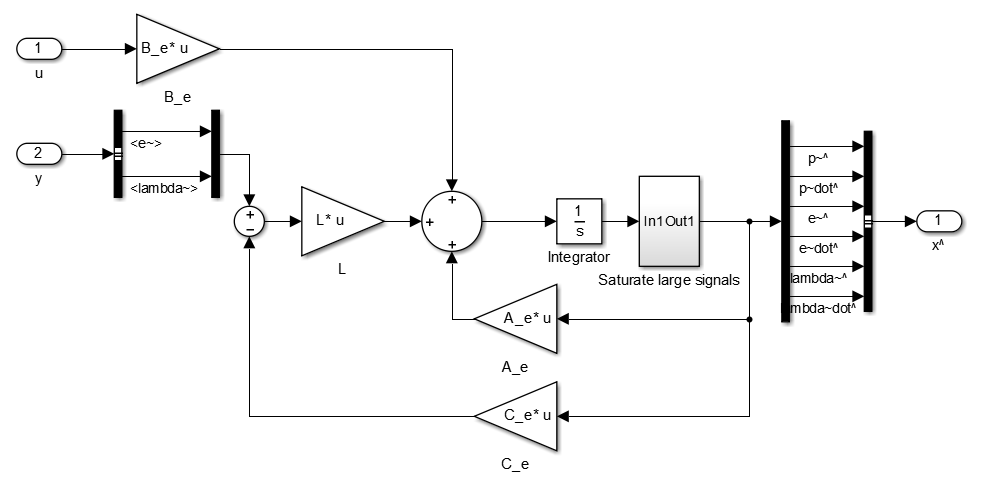
\includegraphics[scale=.6]{images/StateEstimator2States.png}
	\label{fig:Estimator 2 State}
\end{figure}

The observer gain matrix $\bm{L}$ is to be set in such a way that the
poles of the observer are faster than the system, in order to drive the
error to zero.
\begin{figure}[H]
  \caption{ illustrating how to place poles during state, or estimated
    state feedback, on a semi-circle with the same radius, within the
    region shown. \cite{chen14}}
  \label{fig:pole_placement}
  \begin{center}
    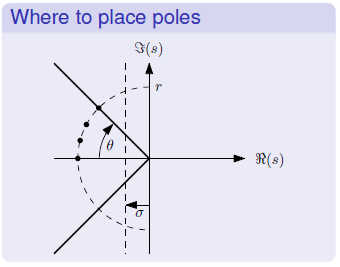
\includegraphics[width=0.5\textwidth]{images/pole_placement}
  \end{center}
\end{figure}
It is recommended that the
poles of the observer be placed as in
\cref{fig:pole_placement}. The real value of the observer poles must be larger
than $\sigma$, which for the observer is the value of the largest real
value of the controlled systems poles. This way, all of the linear
observers poles are such that the observer is faster than the controlled system. $\theta$ is the
largest angle of the observer poles. If this is too large, the system will be underdamped and cause
overshoots in the estimate. However, if the radius is too large, undesired high
frequency noise from the measurements becomes amplified to unwanted
levels. Furthermore, the observer will become increasingly unstable the closer the poles are.

The observer itself has the state space formulation:

\begin{equation*}
  \dot{\hat{\bm{x}}} = \bm{A}\hat{\bm{x}}+\bm{B}\bm{u} + \bm{L}(\bm{y}
  - \bm{C}\hat{\bm{x}})
\end{equation*}
\begin{align*}
  \dot{\bm{e}} &= \dot{\bm{\tilde{x}}} - \dot{\hat{\bm{x}}} \\
               &= \bm{Ax} + \bm{Bu} - \bm{A}\hat{\bm{x}} - \bm{Bu} - \bm{L}(\bm{y}- \bm{C}\hat{\bm{x}}) \\
               &= \bm{A}(\bm{x} - \hat{\bm{x}}) - \bm{L}(\bm{C}\bm{x}- \bm{C}\hat{\bm{x}}) \\
               &= \bm{Ae} - \bm{LCe} \\
\end{align*}
Meaning the error has the state space formulation:
\begin{equation}
  \dot{\bm{e}} = (\bm{A} - \bm{LC})\bm{e}
\end{equation}
As previously stated, for this error to converge to zero the poles of this state space formulation should be placed such that they are
faster than the poles of the system itself. The poles of this state
space system can be placed arbitrarily because $\{\bm{A},\bm{C}\}$ is
observable:
\begin{equation*}
  det(\lambda\bm{I} - \bm{A} +\bm{LC}) = 0
\end{equation*}
For this equation, $\lambda$ are the values that solves the equation,
and also the poles of the observer. By choosing values for $\lambda$,
an $\bm{L}$ emerges in order to make the determinant equal to
zero. The matlab function $place$ places the poles as desired for us:

$\bm{L} = place(\bm{A}^T,\bm{C}^T,\bm{\lambda})^T$, where
$\bm{\lambda}$ is the vector of the observer poles in this instance.

In \cref{fig:LQR_Estimator} the poles are palced on the real line at -20, -40, -60, -80, -100, and -120. This type of observer has minimal overshoot, as there are no complex parts, and the poles are spread far apart to avoid unstable behavior from the observer. Furthermore, the maximum radius is also rather large leading to a fast response. Placing the poles on the real line like this was slightly better than placing them evenly on a circle with radius $r = 60$, and an angle $\theta = 22.5$, because with this pole setup the observer was too oscillatory.

\newgeometry{left=0.5cm,right=0.5cm,top=1cm,bottom=2cm}
\begin{figure}
  \caption{LQR Controller Estimating $p, e$ and $\lambda$}
  \makebox[\textwidth][c]{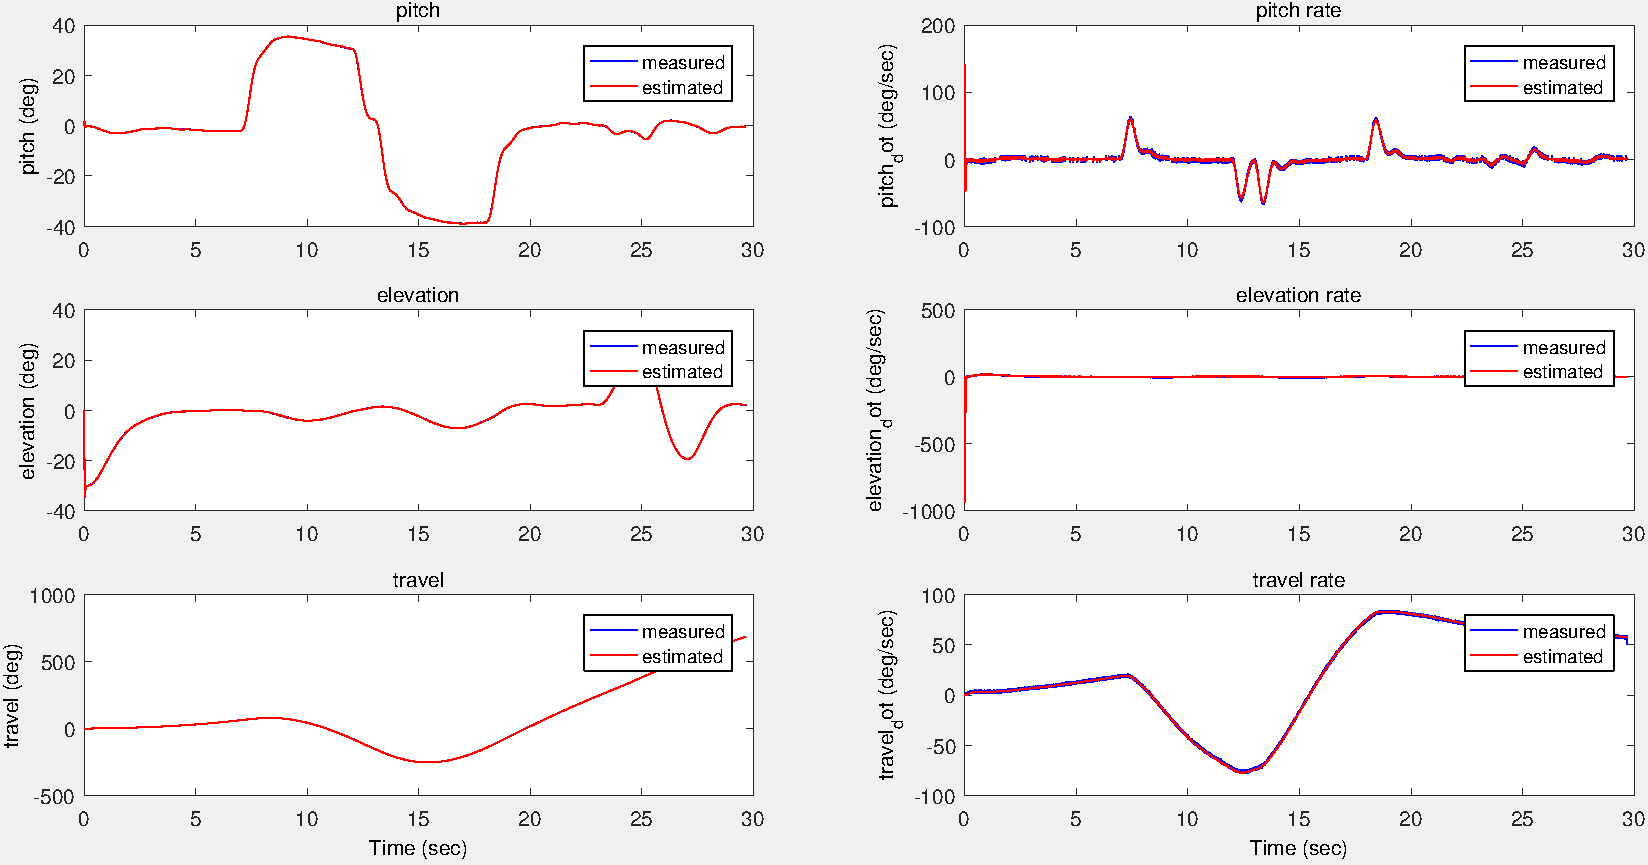
\includegraphics[width = \textwidth]{images/542_LQR_Estimator.pdf}}
  \label{fig:LQR_Estimator}
\end{figure}

\begin{figure}[p]
  \caption{LQR Controller with Integral Effect Estimating $p, e$ and $\lambda$}
  \makebox[\textwidth][c]{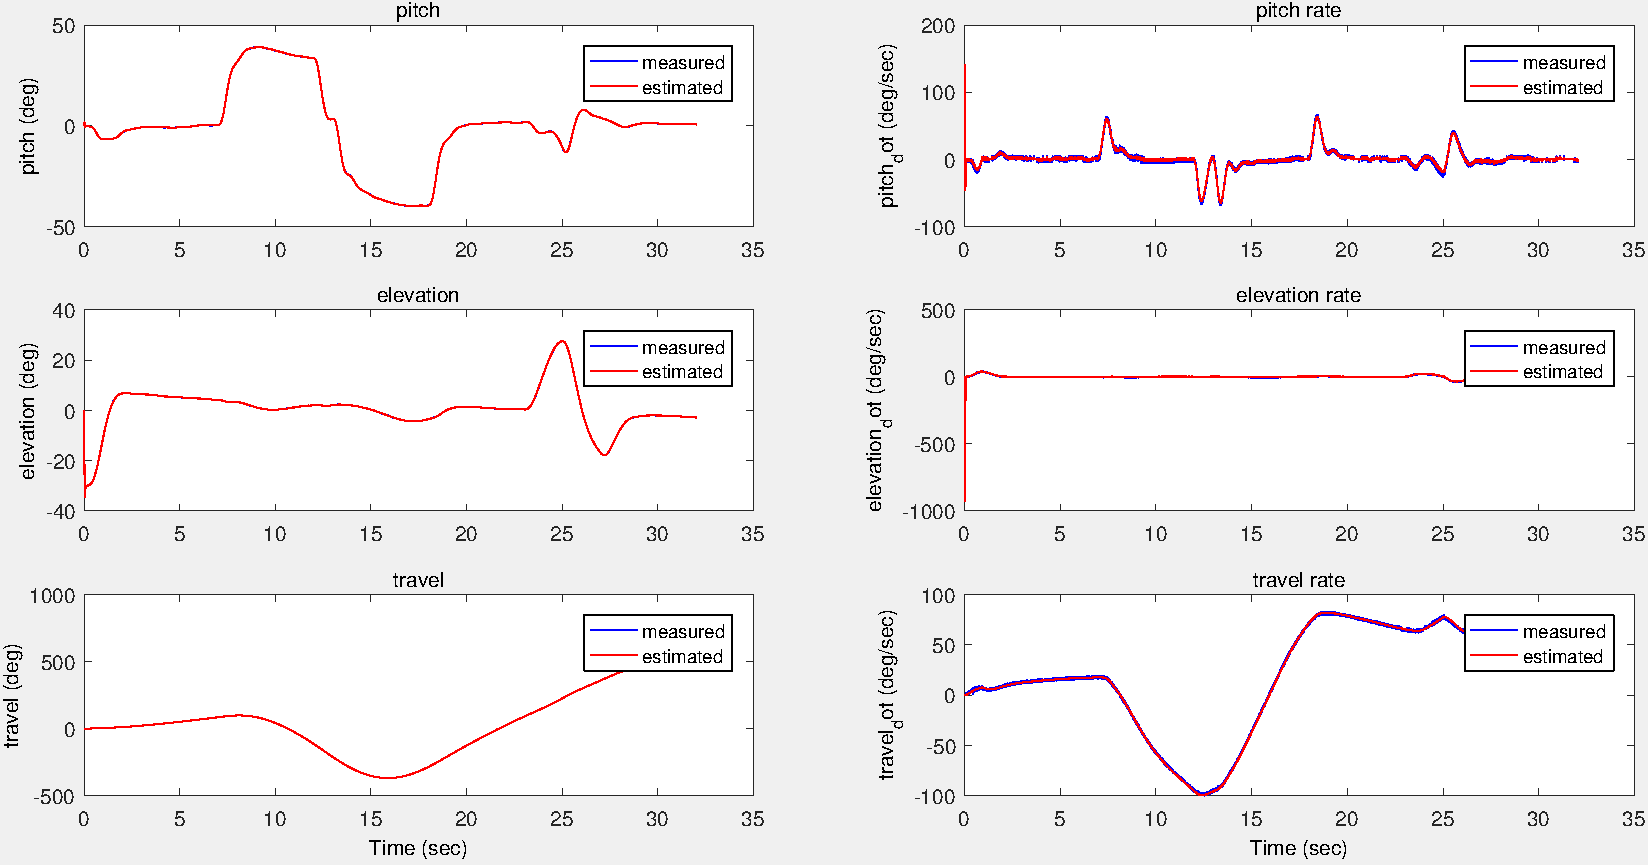
\includegraphics[width = \textwidth]{images/542_LQRIntegralEffect_Estimator.pdf}}
  \label{fig:LQRIntegralEffect_Estimator}
\end{figure}
\restoregeometry

\newgeometry{left=0.5cm,right=0.5cm,top=1cm,bottom=2cm}
\begin{figure}
  \caption{LQR Controller Estimating $p, e$ and $\lambda$}
  \makebox[\textwidth][c]{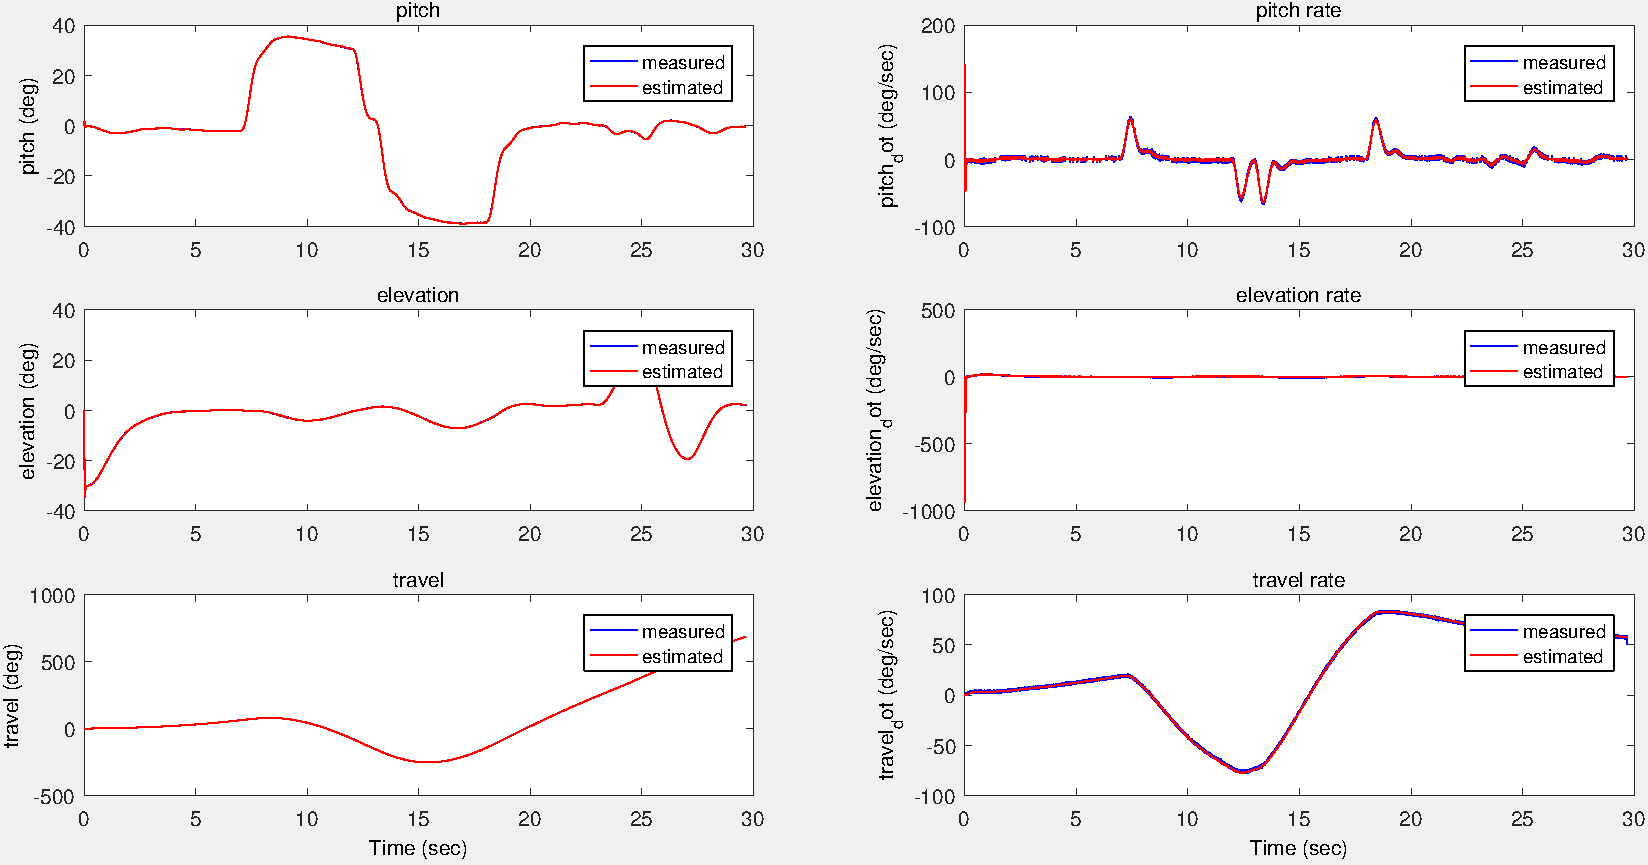
\includegraphics[angle=90, height = \textheight]{images/542_LQR_Estimator.pdf}}
  \label{fig:LQR_Estimator}
\end{figure}

\begin{figure}[p]
  \caption{LQR Controller with Integral Effect Estimating $p, e$ and $\lambda$}
  \makebox[\textwidth][c]{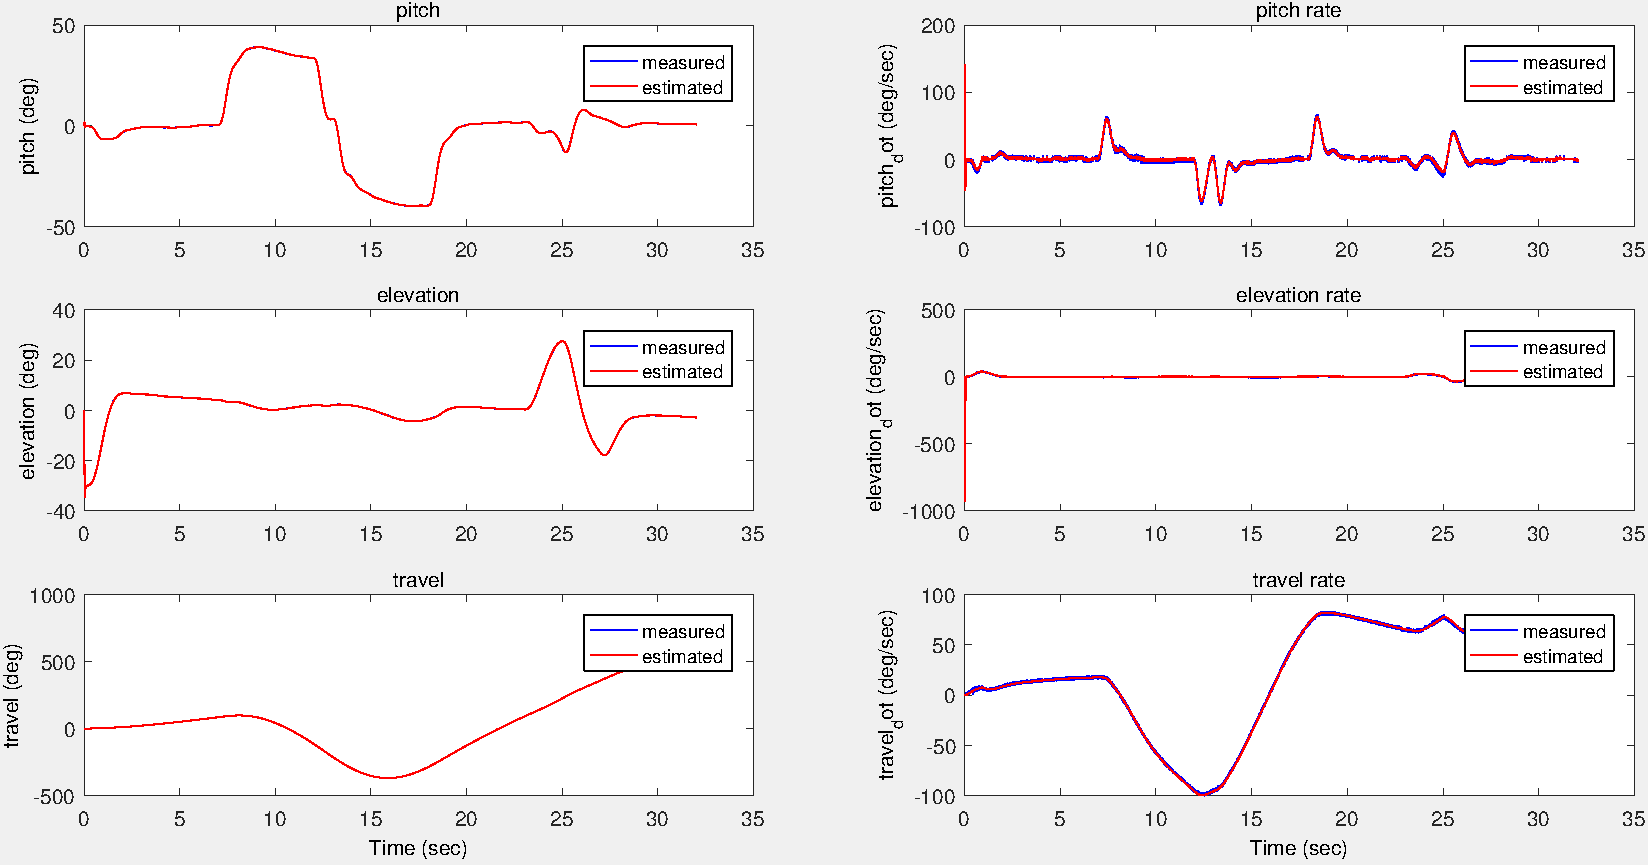
\includegraphics[angle = 90, height = \textheight]{images/542_LQRIntegralEffect_Estimator.pdf}}
  \label{fig:LQRIntegralEffect_Estimator}
\end{figure}
\restoregeometry

\subsection{Problem 3}

When only $\tilde{e}$ and $\tilde{\lambda}$ are measured, the output
matrix becomes:
%
\begin{equation*}
  \bm{C} =
  \begin{bmatrix}
    0 & 0 & 1 & 0 & 0 & 0 \\
    0 & 0 & 0 & 0 & 1 & 0
  \end{bmatrix}
\end{equation*}
%
The observer matrix, found through $obsv(\bm{A},\bm{C})$ is a 12x6
matrix with rank 6. Therefore, it is observable.

However, when only $\tilde{p}$ and $\tilde{e}$ are measured, the
output matrix becomes:
%
\begin{equation*}
  \bm{C} =
  \begin{bmatrix}
    1 & 0 & 0 & 0 & 0 & 0 \\
    0 & 0 & 1 & 0 & 0 & 0
  \end{bmatrix}
\end{equation*}
%
The observer matrix, found through $obsv(\bm{A},\bm{C})$ is a 12x6
matrix with rank 4. Therefore, it is not observable.

This observer is particularly challenging to implement due to the way that pitch is estimated.  The pitch estimate is based on the elevation and travel error of the observer, and the impact of the input $\bm{u}$ on our model and the derivative of the estimated travel rate.  This last term of the pitch estimate becomes a double derivative of measured travel, which significantly amplifies measurement noise.

The observer desirably filters out noise if the poles' negative real value $\sigma$ in \cref{fig:pole_placement} is not too large. However, if this value is too low, the observer becomes too slow and cannot accurately estimate the states. When the double derivation introduces large amounts of noise, the challenge emerges as a balancing act of making $\sigma$ large enough so that the observer accurately estimates the states, while not making it so large that the noise becomes undesirably amplified.

One must also wisely set $\theta$ as seen in \cref{fig:pole_placement} to a high enough value to make the system the right amount of underdamped with not too much oscillation and good settling time, and spread the poles such that they are not close enough to introduce unstable behavior \cite[p.290]{chen14}. It can also help to reduce the poles of the controlled system itself to help make the observer slower in order to counteract the amplified noise while allowing the observer to keep up with the controlled system. This is also limited however, as the controller eventually becomes too slow for efficient control.

In the tuning process, Q and R began at their values from Part 5.4.2, but eventually were reduced to make the controller slower. Many different pole placements for the observer were tried, including on a circle as suggested by Chen, on the real line as was done in 5.4.2 with varying uniform lengths between each pole, on a vertical line with the spread between them decided by $\theta$, and several others \cite[p.290]{chen14}.

What ended up allowing for reasonable control of the system was spreading the poles as much as possible in between the real values of -50 and -3, while keeping $\theta$ as low as possible.  We ended up using poles $\bm{\lambda} = [-3, -20-4i, -20+4i, -30-4i, -30+4i, -50]^T$, $Q = diag([30, 0.1, 50, 1, 15])$, and $R = diag([0.1, 0.1])$.

\newgeometry{left=0.5cm, right=0.5cm, top=1cm, bottom=2cm}
\begin{figure}[h]
\caption{Output using Estimator that measures elevation and travel}
\makebox[\textwidth][c]{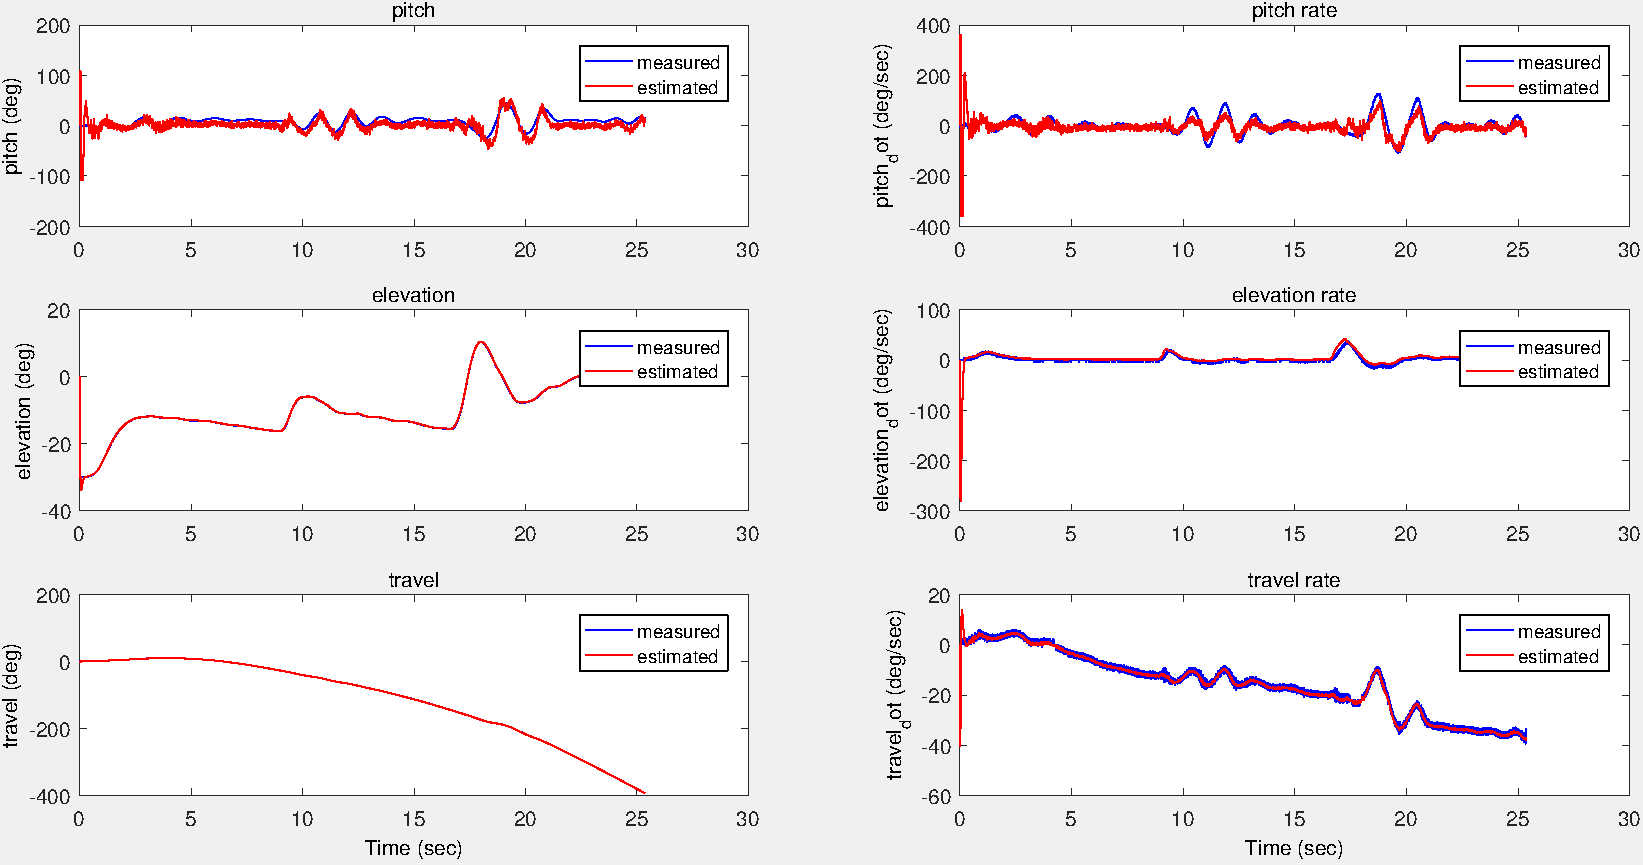
\includegraphics[angle=90, height=\textheight]{images/543_Estimator}}
\label{fig:Estimator4_3}
\end{figure}

%%% Local Variables:
%%% mode: latex
%%% TeX-master: "report_main"
%%% End:
